\documentclass{beamer}
\usepackage{graphicx}
\usetheme{Rochester}

\usepackage[absolute,overlay]{textpos}
\newenvironment{reference}[2]{%
  \begin{textblock*}{\textwidth}(#1,#2)
    \footnotesize\it\bgroup\color{blue!50!black}}{\egroup\end{textblock*}}

\setbeamertemplate{navigation symbols}{}

\title{CPFSK Softwareradio}
\author{Luckas Becker, Tobias Frahm}
\institute[HAW]{Dept. Informations- und Elektrotechnik\\HAW Hamburg}
\date{\today}

\begin{document}

\frame[plain]{\titlepage}

\section[Outline]{}

\frame{\tableofcontents}

\section{Softwareradio}

\frame{
  \frametitle{Softwareradio}
  \begin{itemize}
  \item<1-> Was ist der Unterschied zu einem normalen Empfänger?
  \end{itemize}
}

\section{Signalfluss Empfänger}
\frame{
  \frametitle{Signalfluss Empfänger}
  \begin{columns}
    \begin{column}{0.3\textwidth}
       \begin{itemize}
         \item 1. FIR-Polyphasen Bandpass
         \item 2. komplexes Kammfilter
         \item 3. FM-Verzögerungsdemodulator
         \item 4. Decodierer
       \end{itemize}
    \end{column}
    \begin{column}{0.8\textwidth}
        \begin{center}
         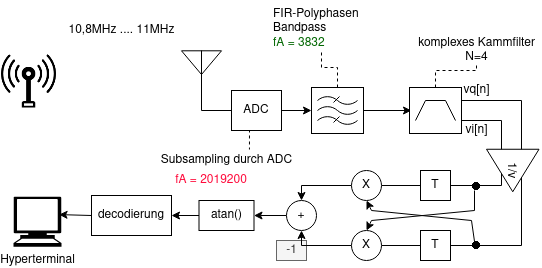
\includegraphics[width=0.6\textwidth]{images/signalfluss.png}
         \end{center}
    \end{column}
  \end{columns}
}

\section{FIR-Polyphasen Bandpass}
\section{Hilbert Transformator}
\section{Komplexes Kammfilter}
\section{FM-Verzögerungsdemodulator}
\section{Decodierer}

\nocite{*} % Include everything in the .bib file.

\bibliographystyle{plainnat}
\bibliography{presentation}

% that's all, folks
\end{document}
